
\documentclass[11pt,a4paper]{article}

\usepackage[utf8]{inputenc} 
\usepackage[T1]{fontenc} 
\usepackage{lmodern}
\usepackage{tcolorbox}

\usepackage[german]{babel}


\setlength{\parindent}{0pt}
\setlength{\parskip}{1ex plus 0.5ex minus 0.5ex}

\usepackage{amsmath} 


\usepackage{graphicx} 

\usepackage[section]{placeins}
\usepackage{booktabs}


\usepackage{hyperref}
\hypersetup{
	colorlinks,
	citecolor=red,
	filecolor=black,
	linkcolor=black,
	urlcolor=black}
\graphicspath{}


\begin{document}



{
	\centering 
	\large 
	Physiklabor für Anfänger*innen \\
	Ferienpraktikum im Sommersemester 2018 \\[4mm]
	\textbf{\LARGE 
		Versuch 19: Gekoppelte Pendel
	} \\[3mm]
	(durchgeführt am 19.09.2018 bei Adrian Hauber) \\
	Ye Joon Kim, Marouan Zouari\\
	\today \\[10mm]
}
\tableofcontents
\section{Einleitung}
Die Bewegung gekoppelter Pendel kann dadurch beschrieben werden, indem man deren Bewegungsgleichungen aufstellen. Es wirken insgesamt zwei Drehmomente auf ein Pendel, die Gravitationskraft $F_G = mg\sin(\varphi)$ (Zur Pendel senkrechte Komponente) und die Federkraft $F_D = D(x_1 - x_2)$. Mit $M = I\ddot{\varphi}$ lautet beide Bewegungsgleichungen:
$$ I \ddot{\varphi_1} = -mg\sin(\varphi_1)L - D(x_1-x_2)l$$
$$I \ddot{\varphi_2} = -mg\sin(\varphi_2)L - D(x_2-x_1)l$$
Mit $x_i = l\sin{\varphi_i}$ mit der Kleinwinkelnäherung sind die Bewegungsgleichungen:
\begin{equation}
\left\{
\begin{array}{c}
I\ddot{\varphi_1}=-mg\varphi_1L - Dl^2(\varphi_1-\varphi_2)
\\
I\ddot{\varphi_2}=-mg\varphi_2L - Dl^2(\varphi_2-\varphi_1)
\end{array}
\right.
\end{equation}

Diese gekoppelte Differenzialgleichungen lassen sich lösen mit einem Variabelaustausch. Nämlich mit $y_1 = \varphi_1 + \varphi_2$ und $y_2 = \varphi_1 - \varphi_2$. Das liefert:
$$\ddot{y_1} = \frac{mgL}{I}y_1$$
$$\ddot{y_2} = \frac{mgL-2Dl^2}{I}y_2$$

Die Pendel wurden als Mathematische Pendel angenähert. Für ein Punktmasse ist sein Trägheitsmoment $I = mr^2$, wobei $r$ der Abstand von dem Rotationsachse zu der Masse ist (In diesem Fall $L$). Eingesetzt in die obigen Formeln liefert:
\begin{equation}
\left\{
\begin{array}{c}
\ddot{y_1} = \frac{g}{L}y_1
\\
\ddot{y_2} = (\frac{g}{L}-\frac{2Dl^2}{mL^2})y_2
\end{array}
\right.
\end{equation}

Beide stellen Gleichungen von Harmonischen Oszillatoren mit den Kreisfrequenzen:
$$ \omega_1^2 = \frac{g}{L}$$
$$ \omega_2^2 = \frac{g}{L}-\frac{2Dl^2}{mL^2} $$

Diese zwei Kreisfrequenzen entsprechen gleich- und gegensinnige Schwingungen. 

\section{Ziel des Versuchs}
Das Ziel des Versuchs ist es, die Schwingungsdauer bei gleich- und gegensinnige Schwingungen sowie die Schwebungsdauer bei verschiedene Kopplungsgrade. 


\section{Aufbau}
Für den Versuch wurden zwei mit einem Feder gebundene Pendel benutzt. Beide Seiten der Feder konnten entlang den Pendel verschoben werden, um den Kopplungsgrad zu ändern. 
\begin{figure} [h]
	\centering
	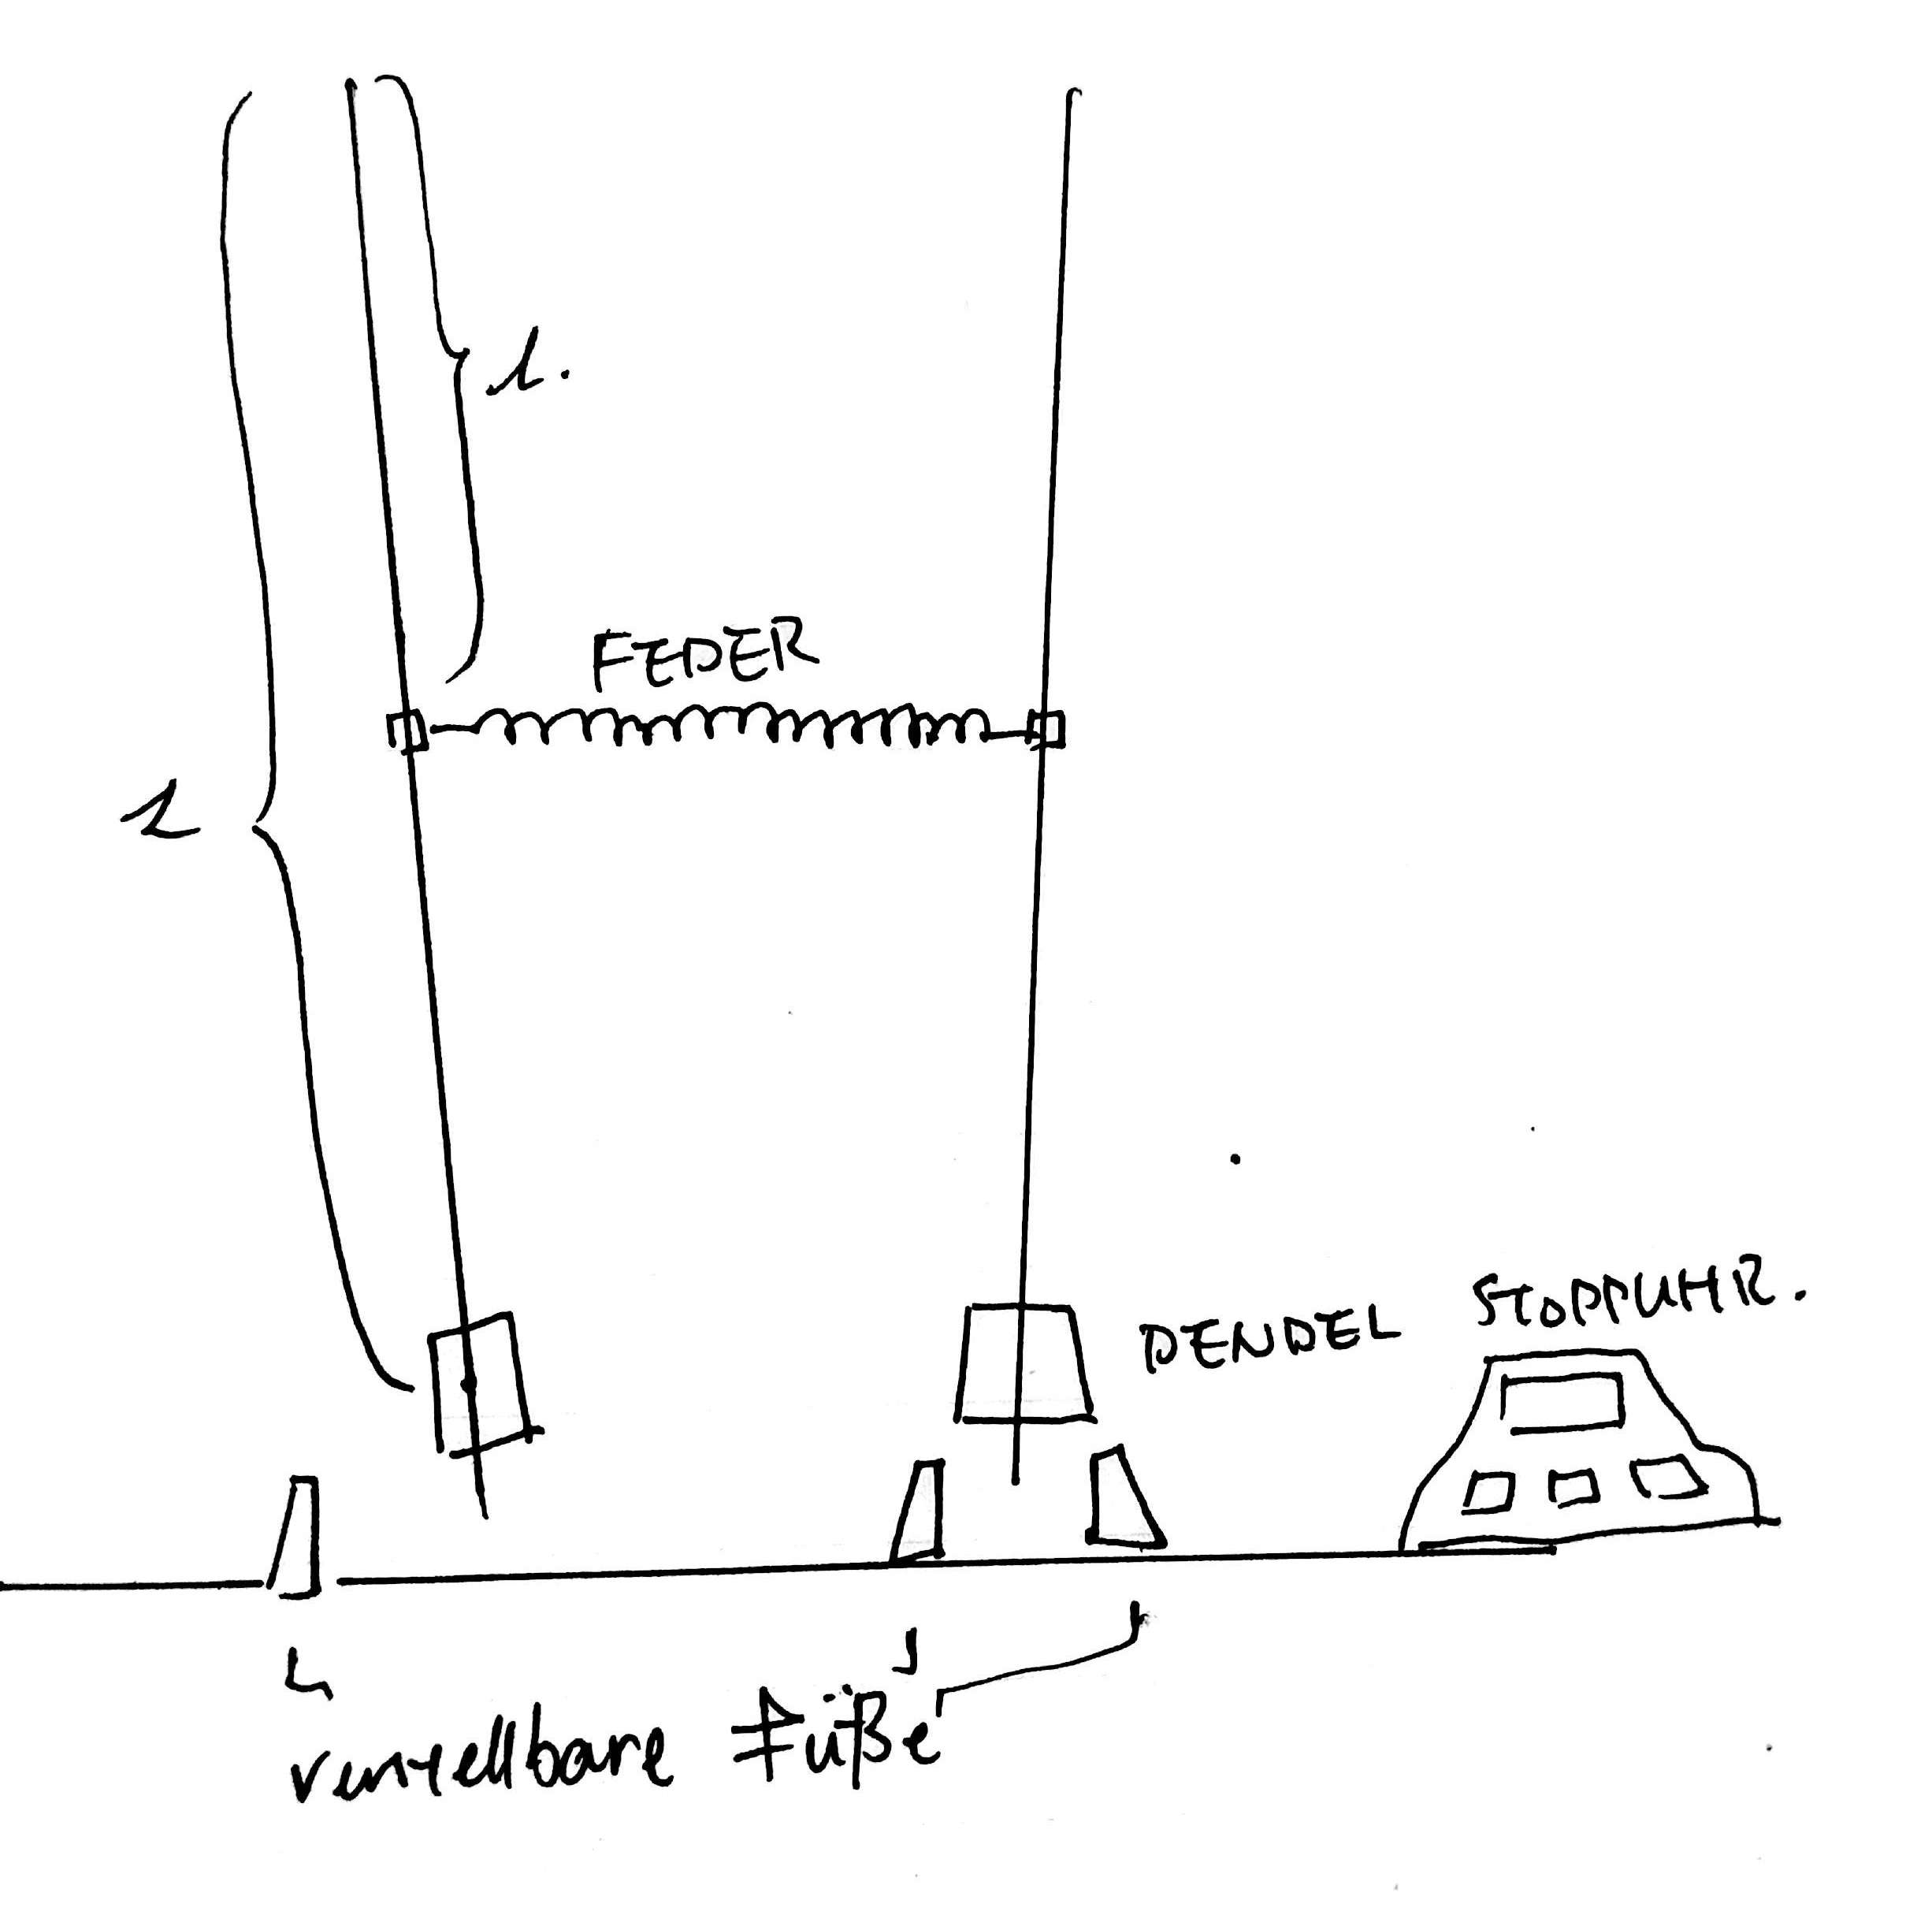
\includegraphics[scale=0.1]{Abb1}
	\caption{Aufbau zum Versuch}
\end{figure}


\section{Durchführung}
Zuerst wurde es sichergestellt, ob die Schwingungsdauer von beiden Pendel die gleiche waren. Die Pendel wurden entkoppelt und die Dauer für vier Schwingungen für beide Pendel wurde mit der Stoppuhr gemessen. Die Positionen der Gewichte an den Pendeln wurden nicht geändert, da zwischen beide Zeitmessungen es fast keinen Unterschied gab (0,06 Sekunde Abweichung).

Danach wurden die beiden Pendel mit der Feder gekoppelt, und beide Pendel wurden in eine Richtung um 4 cm von ihren Ruhelagen mit zwei von den drei verstellbaren Füße verschoben, um die Schwingungsdauer bei gleichsinniger Schwingung zu messen. Die Pendel wurden gleichzeitig losgelassen, indem man die Füße dreht. Die Zeitmessung wurde angefangen, als einer der Pendel schon eine Schwingung gemacht und ihre Wendepunkt erreicht hatte. Es wurde die Zeit für 20 Schwingungen gemessen. Die Pendel wurden dann um 4cm verschoben aber dieses mal in andere Richtungen. Die Zeitmessungen wurden erneut wie oben durchgeführt. 

Für die Messung der Schwebungsdauer wurde nur Pendel um 4cm nach innen verschoben. Die Zeitmessung wurde angefangen, sobald die verschobene Pendel losgelassen wurde. Die Zeit wurde bis dem zweiten Stillstand der anderen Pendel (die ursprünglich an der Ruhelage war) gemessen. Der Prozesse wurde fünfmal wiederholt. 

Die Lage der Feder an den Pendel wurden dann verschoben, um verschiedene Kopplungsgrade einzustellen. Die Schwingungsdauer und Schwebungsdauer wurden wie in den letzten zwei Abschnitte erklärt durchgeführt. Das wurde für vier verschiedene Kopplungsgrade wiederholt. 

\section{Auswertung und Fehleranalyse}
Die Mittelwerte der Schwingungsdauer bei gleichsinnigen Schwingungen, $T_A$, bei gegensinnigen Schwingungen $T_B$, und der Schwebungsdauer $T_S$ für alle Kopplungsgrade und deren Unsicherheiten sind in Tabelle 1 zu sehen. 
\begin{table} [h]
	\begin{tabular*}{0.99\textwidth}{@{\extracolsep{\fill}}c|cccccc}
		\toprule
		$l$ & $T_A$ & $u_{T_A}$ & $T_B$ & $u_{T_B}$ & $T_S$ & $u_{T_S}$  \\
		m & s & s & s & s & s & s   \\
		\bottomrule
		0,705 & 1,63 & 0,02 & 1,874 & 0,009 & 25,4 & 0,3 \\
		0,556 & 1,674 & 0,003 & 1,86 & 0,01 & 33,3 & 0,3 \\
		0,455 & 1,74 & 0,03 & 1,858 & 0,008 & 56,1 & 0,3\\
		0,855 & 1,538 & 0,002 & 1,86 & 0,001 & 18,0 & 0,2 \\
		\bottomrule
	\end{tabular*}
	\caption{Werte für $T_A$, $T_B$ und $T_S$ bei verschiedenen Kopplungsgrade und deren Unsicherheiten.}
\end{table}
\subsubsection{Berechnung}
Um die mittleren Werte für $T_A$ und $T_B$ zu bestimmen wurden die drei Gesamt-Schwingungsdauern summiert und dann durch 60, die totale Anzahl Schwingungen, geteilt. Für deren Unsicherheiten wurde die folgende Formel benutzt:
$$ s_{\bar{x}} = \frac{s_x}{\sqrt{n}}$$
Wobei $s_x$ die Streuung der Mittelwerte ist. Die Streuung der Mittelwerte wurde mit der Formel für Standardunsicherheiten bestimmt, nämlich:
$$s_x=\sqrt{\frac{\sum_{i=1}^{n}(x_i-\bar{x})^2}{n-1}}$$

Die Unsicherheiten der Längen betragen 0,001 m. 

\subsection{Berechnung der theoretischen Schwebungsdauer}
Mit den Werten für $T_A$ und $T_B$ kann der theoretische Wert für $T_S$ berechnet werden, nämlich:
$$\omega_S = \frac{1}{2}(\omega_A-\omega_B)$$
Mit der Substitution $\omega = \frac{2\pi}{T}$ und Umformung lässt sich $T_S$ in Terme von $T_A$ und $T_B$ schreiben:
\begin{equation}
T_S = 2\frac{T_A T_B}{T_B-T_A}
\end{equation}
Die berechnete $T_S$ sind:

\begin{table}[h]
	\centering
	\begin{tabular*}{0.99\textwidth}{@{\extracolsep{\fill}}cccc}
		\toprule
		$l$ & $T_S$ & $u_{T_S}$  \\
		m & s & s   \\
		\bottomrule
		0,705 & 24,6 & 2,6 \\
		0,556 & 33,4 & 1,6 \\
		0,455 & 56 & 14 \\
		0,855 & 17,86 & 0,74 \\
		\bottomrule
	\end{tabular*}
	\caption{Die mit der Formel berechnete Schwebungsdauer für verschiedene Kopplungsgrade}
	\label{tabelle}
\end{table}
Die Unsicherheiten der Werte lassen sich mit der gauß'schen Fehlerfortpflanzung berechnen. Mit:
$$f(T_A,T_B) = 2\frac{T_A T_B}{T_B-T_A}$$ 
sind
$$\frac{\partial f}{\partial T_A} = 2\frac{T_B^2}{(T_A-T_B)^2}$$
$$\frac{\partial f}{\partial T_B} = -2\frac{T_B^2}{(T_B-T_A)^2}$$

Die Unsicherheiten von $T_S$ sind deshalb:
$$u_{T_S} = \sqrt{(\frac{\partial f}{\partial T_A}u_{T_A})^2+(\frac{\partial f}{\partial T_B}u_{T_B})^2}$$

\subsection{Bestimmung der Kopplungsgrade}
Der Kopplungsgrad lässt sich mit der folgenden Formel berechnen:
\begin{equation}
K = \frac{T_B^2-T_A^2}{T_B^2+T_A^2}
\end{equation}

Die berechnete Werte dafür für jede Messreihe und deren Unsicherheiten sind:

\begin{table}[h]
	\centering
	\begin{tabular*}{0.99\textwidth}{@{\extracolsep{\fill}}cccc}
		\toprule
		$l$ & $K$ & $u_{K}$  \\
		m &  &    \\
		\bottomrule
		0,705 & 0,14 & 0,01 \\
		0,556 & 0,105 & 0,005 \\
		0,455 & 0,06 & 0,02 \\
		0,855 & 0,187 & 0,008 \\
		\bottomrule
	\end{tabular*}
	\caption{Die mit der Formel berechnete Schwebungsdauer für verschiedene Kopplungsgrade}
	\label{tabelle}
\end{table}

Die Unsicherheiten lassen sich wiederum mit der gauß'schen Fehlerfortpflanzung berechnen mit:
$$f(T_A,T_B) = \frac{T_B^2-T_A^2}{T_B^2+T_A^2}$$
sind
$$\frac{\partial f}{\partial T_A} = -\frac{4T_A T_B^2}{(T_A^2+T_B^2)^2}$$
$$\frac{\partial f}{\partial T_B} = \frac{4T_A^2 T_B}{(T_B^2+T_A^2)^2}$$
Die Unsicherheiten von $K$ sind deshalb:
$$u_{K} = \sqrt{(\frac{\partial f}{\partial T_A}u_{T_A})^2+(\frac{\partial f}{\partial T_B}u_{T_B})^2}$$

Eine lineare Regression wurde dann gemacht, um zu sehen, ob es eine lineare Zusammenhang gibt zwischen $l^2$ und $K$. Die lineare Gleichung lautet:
$$ K = a\cdot l^2 +b = 0,2327 l^2 + 0,02 $$
Mit den Unsicherheiten: $u_a = 0,01$ und $u_b = 0,03$ (Siehe Abbildung). 
\begin{figure}[h]
	\centering
	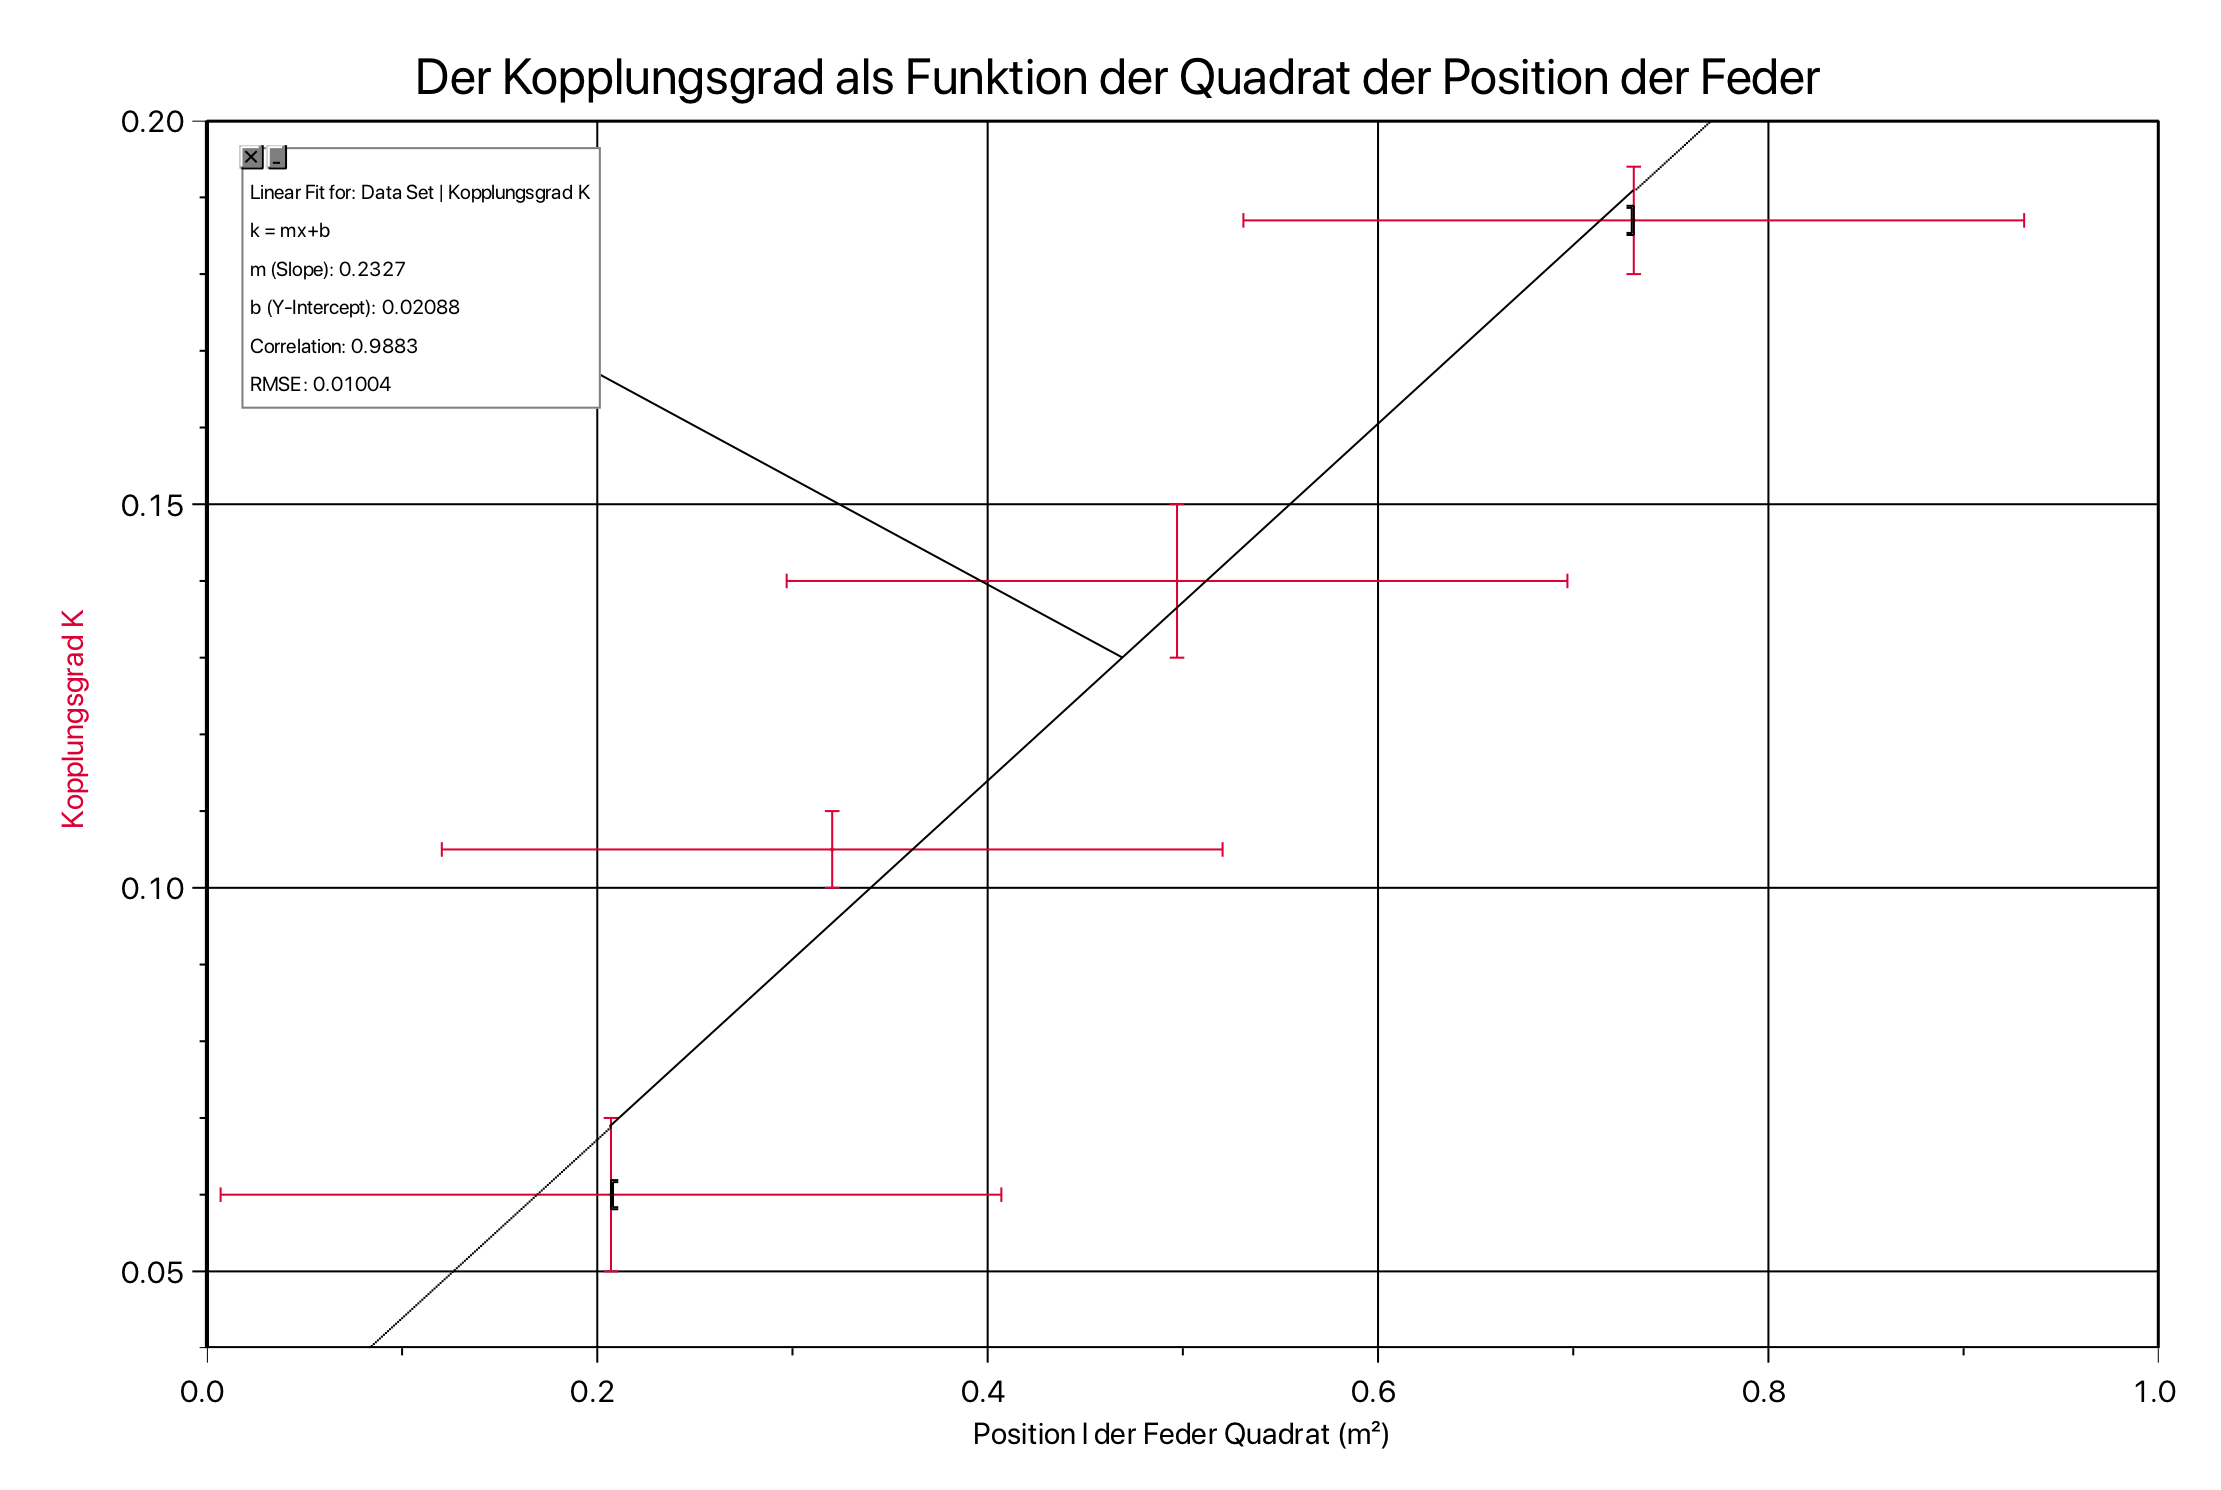
\includegraphics[width=\textwidth]{Abb2}
	\caption{Eine Graph von $K$ als Funktion von $l^2$}
\end{figure}

\section{Diskussion der Ergebnisse}

\section{Literatur}

\section{Anhang}





\end{document}